% MIT License

% Copyright (c) 2022-2023 Melonbob (Robert F. Burgie) <brew.Melonbob@mac.com>

% Permission is hereby granted, free of charge, to any person obtaining a copy
% of this software and associated documentation files (the "Software"), to deal
% in the Software without restriction, including without limitation the rights
% to use, copy, modify, merge, publish, distribute, sublicense, and/or sell
% copies of the Software, and to permit persons to whom the Software is
% furnished to do so, subject to the following conditions:

% The above copyright notice and this permission notice shall be included in all
% copies or substantial portions of the Software.

% THE SOFTWARE IS PROVIDED "AS IS", WITHOUT WARRANTY OF ANY KIND, EXPRESS OR
% IMPLIED, INCLUDING BUT NOT LIMITED TO THE WARRANTIES OF MERCHANTABILITY,
% FITNESS FOR A PARTICULAR PURPOSE AND NONINFRINGEMENT. IN NO EVENT SHALL THE
% AUTHORS OR COPYRIGHT HOLDERS BE LIABLE FOR ANY CLAIM, DAMAGES OR OTHER
% LIABILITY, WHETHER IN AN ACTION OF CONTRACT, TORT OR OTHERWISE, ARISING FROM,
% OUT OF OR IN CONNECTION WITH THE SOFTWARE OR THE USE OR OTHER DEALINGS IN THE
% SOFTWARE.
\documentclass{article}
\usepackage[letterpaper,portrait]{geometry}
\pagenumbering{gobble}
\usepackage{pgfplots,textcomp}
\pgfplotsset{width=12cm,compat=1.15}
\begin{document}
% 6-step: acid rest mash-in; 2INF-modRIMS protein rest; 3DEC-modRIMS; 4INF-modRIMS beta rest; 5INF-modRIMS alpha rest; 6DEC-modRIMS mash-out
% a-TR-I-D-TR-I-TR-I-TR-D-TR
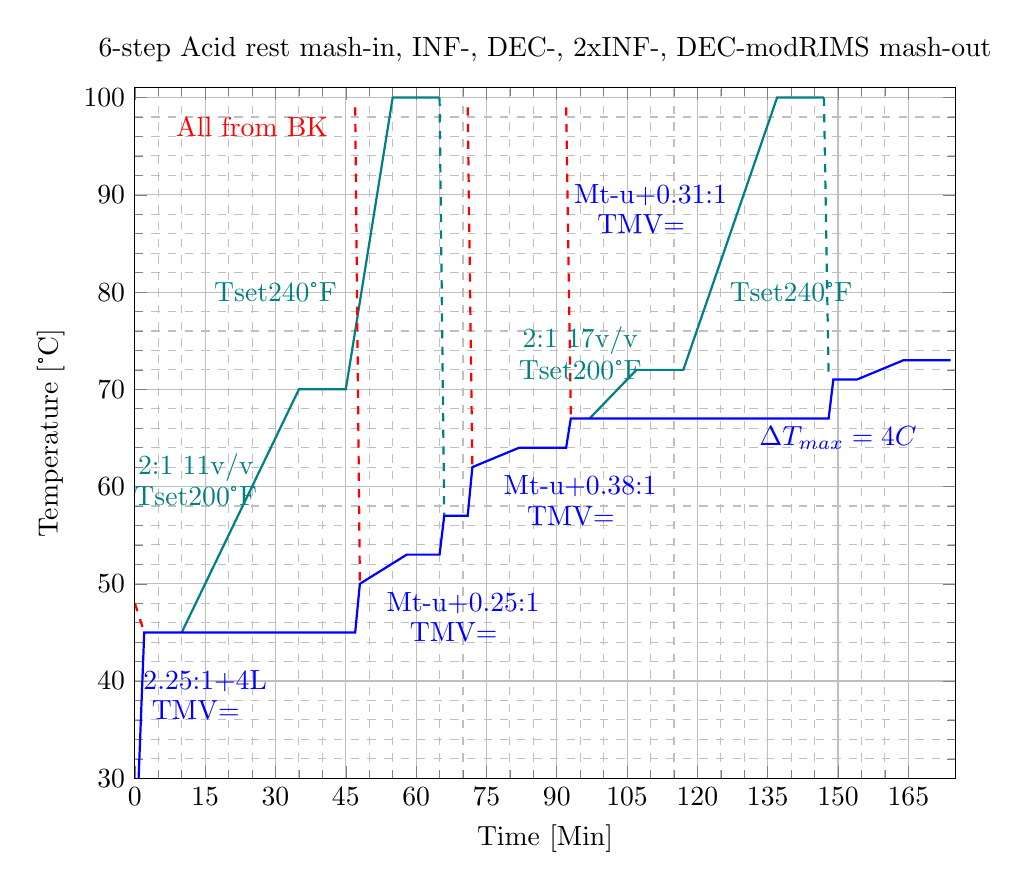
\begin{tikzpicture}
\begin{axis}[
  title={6-step Acid rest mash-in, INF-, DEC-, 2xINF-, DEC-modRIMS mash-out},
  xlabel={Time [Min]},
  ylabel={Temperature [\textdegree{C}]},
  xmin=0, xmax=175,
  ymin=30, ymax=101,
  xtick={0,15,30,45,60,75,90,105,120,135,150,165},
  ytick={30,40,50,60,70,80,90,100},
  % legend pos=north west,
  ymajorgrids=true,
  xmajorgrids=true,
  grid style=thin,
  %grid=major,
  minor grid style=dashed,
  yminorgrids=true,
  xminorgrids=true,
  yminorticks=true,
  xminorticks=true,
  minor y tick num=4,
  minor x tick num=2
]
\addplot [color=red, style=dashed,thick]
  coordinates {
    (0,48)% strike temp
    (2,45)% mash-in 2.25:1 (36+4L on PR1 w/ 16kg) TMV=40+0.67*16=51L
  };
\node [color=blue] at (axis cs:15,40) {2.25:1+4L};
\node [color=blue] at (axis cs:13,37) {TMV=   };
\addplot [color=teal, style=thick]
  coordinates {
    (10,45)% 3DEC heat 6L thick (2:1 11v/v)
    (35,70)% 1C/min (induction set 200F) then
    (45,70)% 10' decoction rest until starch neg
    (55,100)% 3DEC 3C/min (induction set 240F)
    (65,100)% boil 10 min
  };
\addplot [color=red, style=dashed,thick]
  coordinates {
    (47,99)(48,50)% 2INF 0.25:1 (4L on PR1 w/ 16kg) TMV=55L
  };
\node [color=teal] at (axis cs:13,62) {2:1 11v/v};
\node [color=teal] at (axis cs:13,59) {Tset200\textdegree{F}};
\node [color=teal] at (axis cs:30,80) {Tset240\textdegree{F}};
\addplot [color=teal, style=dashed,thick]
  coordinates {
    (65,100)(66,57)% recombine
  };
\node [color=red] at (axis cs:25,97) {All from BK};
\node [color=blue] at (axis cs:70,48) {Mt-u+0.25:1 };
\node [color=blue] at (axis cs:68,45) {TMV=   };
\addplot [color=red, style=dashed,thick]
  coordinates {
    (71,99)(72,62)% 4INF 0.38:1 (6L on PR1 w/ 16kg) TMV=61L
  };
\node [color=blue] at (axis cs:95,60) {Mt-u+0.38:1 };
\node [color=blue] at (axis cs:93,57) {TMV=   };
\addplot [color=red, style=dashed,thick]
  coordinates {
    (92,99)(93,67)% 5INF 0.31:1 (5L on PR1 w/ 16kg) TMV=66L
  };
\node [color=blue] at (axis cs:110,90) {Mt-u+0.31:1 };
\node [color=blue] at (axis cs:108,87) {TMV=   };
\addplot [color=teal, style=thick]
  coordinates {
    (97,67)% 6DEC heat 11L thick (2:1 17v/v)
    (107,72)% 1C/2min (induction set 200F) then
    (117,72) % 10' decoction rest until starch neg
    (137,100)% 6DEC 3C/2min (induction set 240F)
    (147,100)% boil 10 min
  };
\node [color=teal] at (axis cs:95,75) {2:1 17v/v};
\node [color=teal] at (axis cs:95,72) {Tset200\textdegree{F}};
\node [color=teal] at (axis cs:140,80) {Tset240\textdegree{F}};
\addplot [color=teal, style=dashed,thick]
  coordinates {
    (147,100)(148,71)% recombine
  };
\node [color=blue] at (axis cs:150,65) {$ \Delta T_{max}=4C $};
\addplot [color=blue, style=thick]
  coordinates {
    (0,20)% initial grist temp
    (2,45)% mash-in, 5 min rest, DEC pulled
    (42,45)% 45' acid rest, no loss with RIMS
    (47,45)%
    (48,50)% 2INF 0.25:1 4L on PR1
    (58,53)% TmodRIMS 1C/3min
    (65,53)% 7' protein rest, no loss with RIMS, w/o cooling loss -4C/hr=-1C/15min
    (66,57)% 3DEC recombined
    (71,57)% 5' Dextrin rest
    (72,62)% 4INF 0.38:1 6L on PR1
    (82,64)% TmodRIMS 1C/5min in beta
    (92,64)% 10' TmodRIMS in beta
    (93,67)% 5INF 0.31:1 5L on PR1
    (98,67)% 5' alpha rest, no cooling loss w/ RIMS, DEC pulled
    (148,67)% 50' TmodRIMS in alpha, no cooling loss w/ RIMS
    (149,71)% 6DEC recombined 
    (154,71)% 5' hi-alpha TmodRIMS until starch negative
    (164,73)% TmodRIMS 1C/5min mash-out
    (169,73)% 5' Lauter/ mash bed settle/ no RIMS
    (174,73)% 5' Vorlauf/ no hose
  };
% \legend{}
 
\end{axis}
\end{tikzpicture}
\end{document}